
                \documentclass{standalone}
                \usepackage{tikz}
                \usepackage{standalone}
                \usetikzlibrary{calc}
                \begin{document}
                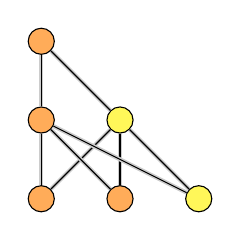
\begin{tikzpicture}\node[circle, draw=black, draw=black, fill=orange!65] (0) at (0, 0) {};\node[circle, draw=black, draw=black, fill=orange!65] (1) at (1, 0) {};\node[circle, draw=black, draw=black, fill=yellow!65] (2) at (2, 0) {};\node[circle, draw=black, draw=black, fill=orange!65] (3) at (0, 1) {};\node[circle, draw=black, draw=black, fill=yellow!65] (4) at (1, 1) {};\node[circle, draw=black, draw=black, fill=orange!65] (5) at (0, 2) {};\draw[line width=1.5pt,-,black!20] (0) -- (3);\draw[draw,-] (0) -- (3);\draw[line width=1.5pt,-,black!20] (0) -- (4);\draw[draw,-] (0) -- (4);\draw[line width=1.5pt,-,black!20] (1) -- (3);\draw[draw,-] (1) -- (3);\draw[line width=1.5pt,-,black!20] (1) -- (4);\draw[draw,-] (1) -- (4);\draw[line width=1.5pt,-,black!20] (2) -- (3);\draw[draw,-] (2) -- (3);\draw[line width=1.5pt,-,black!20] (2) -- (4);\draw[draw,-] (2) -- (4);\draw[line width=1.5pt,-,black!20] (3) -- (5);\draw[draw,-] (3) -- (5);\draw[line width=1.5pt,-,black!20] (4) -- (5);\draw[draw,-] (4) -- (5);
                \end{tikzpicture}
                \end{document}